Since the learning process that involves the human-computer interaction takes a regular amount of episodes in order to generate results, automated policies where used during training in order to test the functionality of our algorithm. For example, one of the policies that we applied in order to test if our algorithm was learning correctly, was to tell it \emph{not to play any note with a frequency higher than the previous note}. In other words, always play a note with lower pitch that the previous one. In musical terms, what this is trying to teach is a descendant scale. For that, we gave a $ -100 $ reward in case the algorithm played a note higher than the previous one, and a $ +10 $ if it played a note lower than the previous one. We could see that our algorithm was able to learn the optimal policy after $ 1500 $ iterations in average.

\begin{figure}[h]
  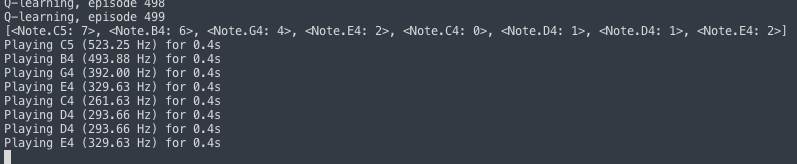
\includegraphics[width=\linewidth]{it500.jpg}
  \caption{Iteration 500: Not efficient policy due to note transitions like C4 to D4 in position 5}
  \label{fig:it500}
\end{figure}

As we can see in Figure \ref{fig:it500}, the optimal policy was not found yet, since the algorithm is still deciding to use a higher note in the position 6 than the previous note (position 5).

\begin{figure}[ht]
  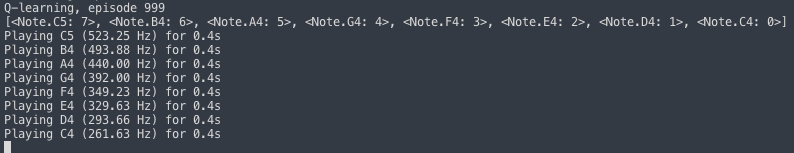
\includegraphics[width=\linewidth]{it1000.png}
  \caption{Iteration 1000: Optimal policy. Each note is lower than the previous one.}
  \label{fig:it1000}
\end{figure}

In Figure \ref{fig:it1000} we notice that the algorithm finally found the optimal policy for the scenario that we proposed (each note should be lower than the previous one). Of course, this condition does not have any musical validity, it was only used for testing the learning capability of our algorithm.

